\documentclass{www2010-submission}

\usepackage{graphicx}
% \usepackage[left=2cm,top=1cm,right=3cm]{geometry}

\begin{document}
\setlength{\parindent}{0pt}
\setlength{\parskip}{.5ex plus 0.5ex minus 0.2ex}


% \setlength{\parskip}{8pt}
% \setlength{\parsep}{8pt}


\title{ drawnTogether -- a collaborative approach to virtual graffiti }

\author{ Jeremy Kelley, Kyumin Lee, \& Xiheng Zhang }

\date{\today}

\maketitle

\section{ Ethnographic data gathering }
We conducted three semi-structured interviews and carried out at least five
other free form conversations around the goals of the project.  Since graphics
creation on mobile devices is very infantile, we instead chose to focus on
``normal users'' that may have used graphics programs and the intersection with
their mobile usage.

The three researchers in this project were to each speak with individuals and
gather information concerning artistic leanings and computer based tools used
in these endeavors.  In hindsight, we should have either had one individual
conduct all interviews, or provided a more rigid script for each interviewer to
use.  The questions started from the following set, but would often stray into
other tangents concerning the topic:

\begin{itemize}
\item Can you list any devices you have used for drawing besides paper?
\item Have you used any drawing software before?
	\begin{itemize}
	\item If yes, which tool have you used and how often have you used it? 
	\item Would you choose to use Paint or Photoshop if familiar with both?
	\end{itemize}
\item Do you prefer art creation on paper or via digital means?  Why?
\item Have you ever considered collaborating with others when creating artistic works?
\item Imagine you are able to draw on a screen and have that work appear on a
	building.  What would you draw?
\end{itemize}

These questions, although not rigidly adhered to, provided for interesting
conversation starters and were definitely useful in showing a definite interest
in our eventual application.

One of the interviewees came from China and is a student at Texas A\&M
University.  He mentioned he usually uses Paint application and sometimes uses
Photoshop and that, overall, he uses graphics applications about once a month.
His responses indicated that the MS Paint application is simple and easy to
use, and that Photoshop has too many functions and is quite sophisticated to
use.  Additionally, after he heard about our application, he said it would be
helpful to provide a function to search a sketch drawn by friends without going
to a certain location.

One of a the respondents, an economics student of Chinese origins, has never used an
iPhone before.  Yet, she is very interested in drawing and painting.  She
mentioned highly enjoying drawing on a small toy board which has an eraser as 
a child.  She randomly uses the Windows Paint application, as well.  Most often
though, she uses analysis software, such as SPSS to draw professional diagrams.
When questioned about pure artistic endeavors, she expressed a high preference
pen and a paper drawing and a complete disdain for using a mouse to draw strokes
when sketching. Her response concerning this area was ``If I can have a pen to
draw on the computer screen, I would definitely draw a good picture.''
Concerning collaboration, she definitely showed some excitable interest but her
biggest concern was the ability to tell her strokes apart from others.   When
the question about drawing on a screen and appearing on a building was
broached, she replied that she would like to draw something related to her
surroundings and that she would care about others sketches.  In particular, she
remarked, ``That's one aspect of collaboration, right? First, I care about my
friends' drawing. Then people who share the same interests with me.'' 
When our intended application was finally revealed, she said she would care
more about what people around her were drawing.

Another interviewee, a technology worker from Houston, TX, mentioned being
highly proficient in multiple graphics applications, including Photoshop.
Throughout the interview, his mind raced with different ways to collaborate on
different projects even at one point asking ``Would it be possible to really
project what others were drawing onto an external wall for live events and
concerts?''  This was an idea previously not considered by the researchers and
one that is being heavily considered as a way of involving passersby who may
not have a device but could still be considered consumers of collaborative
creations.

\section{Storyboards}
We can apply our application to various scenarios. In this section, we show two
of them.  Storyboards for the intended applicaiton 

\subsection{Scenario 1: collaborative drawing}

Alice and Bob are students at Texas A\&M University and are friends. Alice
wanted to draw the MSC building before it is remodeled, so she went near to the
building and sketched it using our application. She did not finish the drawing
because of a class. While she is going to a classroom, she sends a SMS message
to Bob. The message is ``Could you finish the sketch for the MSC building in
location X?'' Fortunately, he is passing in front of the building and starts to
add some sketch into the figure, which Alice drew. Sometimes later, he finishes
to draw the building and sends a SMS message to her. The message is ``I'm
done!'' After the class is finished, she goes to the location in which she drew
the building. She can view what they drew and is satisfied about what they did.
This can be weakly seen in Figure \ref{fig:s1}.

\subsection{scenario 2: event impressions}

Alice and Bob can attend a public event, such as a conference or a concert.
While at the event, each user contributes small sketches to the location.  On a
whim, Alice decides to draw the standing position of each speaker during their
talk or show and tags these creations as ``position''.  Likewise, Bob decides
that each time a question is asked from the audience, he will annotate that by
creating a mark on the screen and tagging it ``question''.  At the end of the
conference, they each view the other's visual notes and deduce several
anecdotal observations related to audience participation and performer
position.  This can be weakly seen in Figure \ref{fig:s2}.

\begin{figure}
\centering
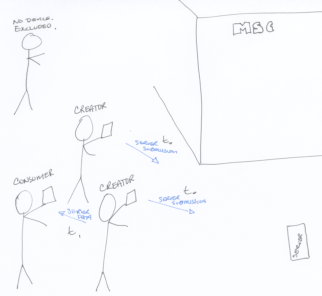
\includegraphics[width=.50\textwidth]{scen1.pdf}
\caption{Scenario 1} \label{fig:s1}
\end{figure}

\begin{figure*}
\centering
\includegraphics[width=.80\textwidth]{scen2.pdf}
\caption{Scenario 2} \label{fig:s2}
\end{figure*}


%%%%%%%%%%%%%%%%%%%
% \bibliographystyle{plain}
% \bibliography{../bibli} 
\end{document}
